\documentclass[border=0.2cm, convert={density=600}]{standalone}
 
% Required packages and libraries
\usepackage{tikz}
\usetikzlibrary{shapes}
 
\begin{document}
 
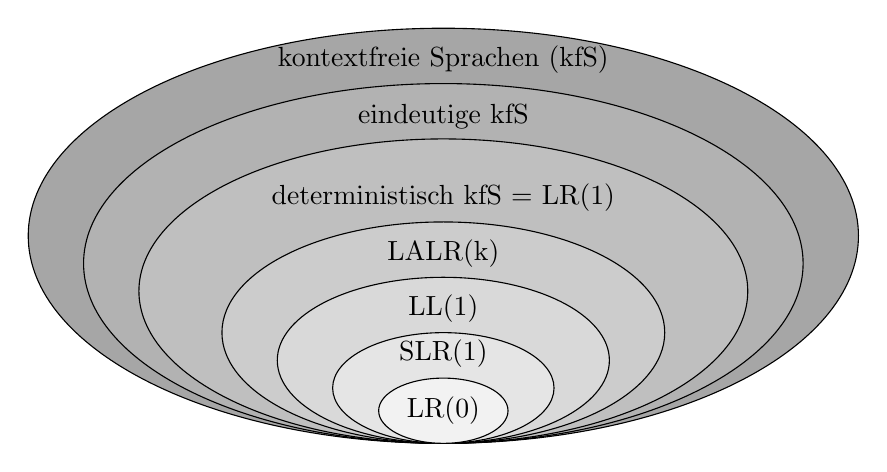
\begin{tikzpicture}
\node[above,ellipse,minimum height=15em,minimum width=30em,draw,fill=black!35] (g) {};
\node[above,ellipse,minimum height=13em,minimum width=26em,draw,fill=black!30] (f) {};
\node[above,ellipse,minimum height=11em,minimum width=22em,draw,fill=black!25] (e) {};
\node[above,ellipse,minimum height=8em,minimum width=16em,draw,fill=black!20] (d) {};
\node[above,ellipse,minimum height=6em,minimum width=12em,draw,fill=black!15] (c) {};
\node[above,ellipse,minimum height=4em,minimum width=8em,draw,fill=black!10] (b) {};
\node[above,ellipse,minimum height=2em,minimum width=4em,draw,fill=black!5] (a) {LR(0)};
\path (a.north) node[above] {SLR(1)}
      (b.north) node[above] {LL(1)}
      (c.north) node[above] {LALR(k)}
      (d.north) node[above] {deterministisch kfS = LR(1)}
      (e.north) node[above] {eindeutige kfS}
      (f.north) node[above] {kontextfreie Sprachen (kfS)}
      ;
\end{tikzpicture}
 
\end{document}